% !TEX root = /media/ueslei/Ueslei/INPE/PCI/Projetos/Guia_COAWST/main.tex
\chapterimage{header.jpg}
\chapter{Building the weights between grids with SCRIP}
\bigskip
\section{Building the weights}
\bigskip
 As seen in the section \textcolor{bleu_cite}{\ref{scripsecao}}, SCRIP is used to interpolate the weights between two or more grids of different models. 
In COAWST, the package was modified to generate only one NetCDF file that will be used during integrations.
\bigskip

 The SCRIP directory is located at:
\bigskip

\begin{bashcode}
/home/name.surname/COAWST/Lib/SCRIP
\end{bashcode}
\bigskip

 Inside the folder, look for the file with the extension\textit{.in}. As in the example in Figure \textcolor{bleu_cite}{\ref{scripinnedit}}:

\begin{figure}[H]
    \centering
    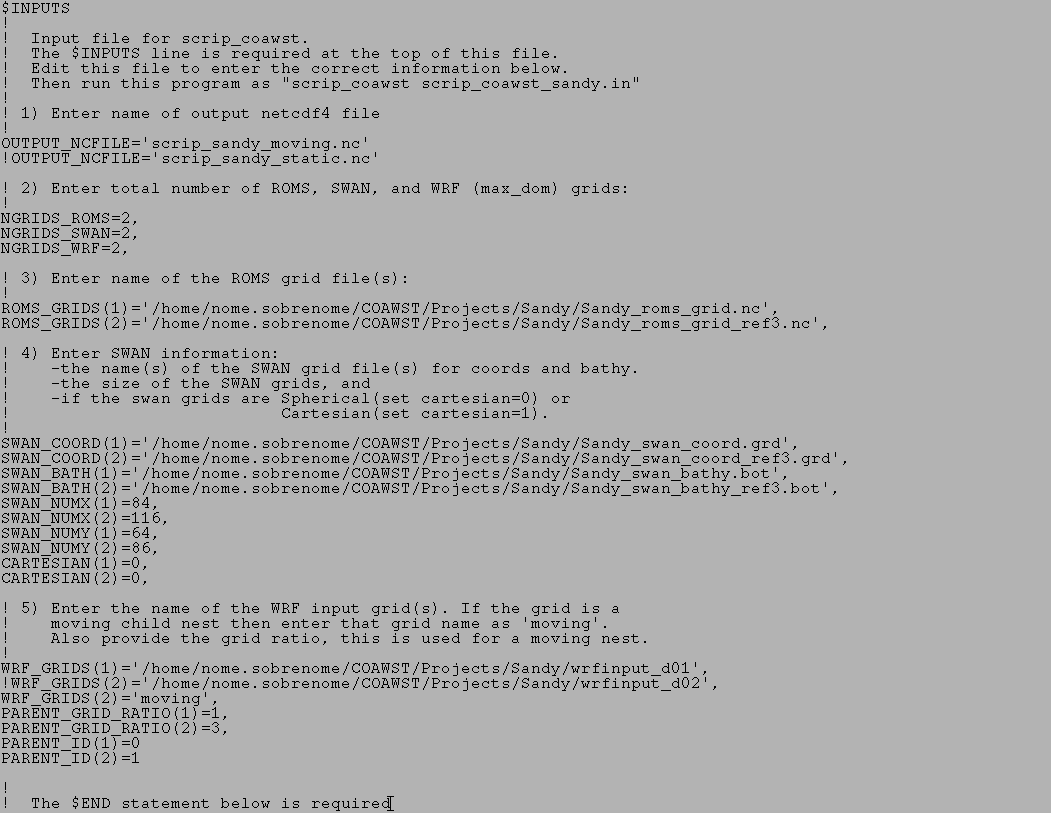
\includegraphics[width=0.65\textwidth]{scripin.png}
    \caption{SCRIP \textit{.in} file for the Sandy project.}
    \label{scripinnedit}
\end{figure}
\bigskip

 In \textit{OUTPUT\_NCFILE}, change the name of the NetCDF file that will be generated, if necessary.
\bigskip

 In section 2 of the file, change the variables \textit{NGRIDS\_ROMS}, \textit{NGRIDS\_SWAN} and \textit{NGRIDS\_WRF} according to the number of grids, 
existing in your project, in ROMS, SWAN and WRF, respectively.
\bigskip

 In the third section of the file, renew the ROMS grid directories according to the names in your project.
\bigskip

 In the fourth section, in addition to changing the directories of the SWAN grids (\textit{SWAN\_COORD} and \textit{SWAN\_BATH}), change the 
number of existing grid points, in the variables \textit {SWAN\_NUMX} and \textit{SWAN\_NUMY}.
\bigskip

 Finally, in the fifth section, change the WRF grid directories (\textit{WRF\_GRIDS}). In \textit {PARENT\_GRID\_RATIO}, if your project includes nesting 
between the WRF grids, change to the relationship used between the grids used in your project. In \textit{PARENT\_ID}, add the grid ID.
\bigskip

 Then, save the changes.
\bigskip

 To run SCRIP, search the repository for the file \textit{qsub\_scrip.sh}:
\bigskip

\begin{bashcode}
/home/name.surname/repositorio/qsub_scrip.sh
\end{bashcode}
\bigskip

 Move the file to the SCRIP directory:
\bigskip

\begin{bashcode}[fontsize=\scriptsize]
mv /home/name.surname/repositorio/qsub_scrip.sh /home/name.surname/COAWST/Lib/SCRIP
\end{bashcode}
\bigskip

 Open the file \textit{qsub\_scrip.sh}:
\bigskip

\begin{bashcode}
nedit qsub_scrip.sh
\end{bashcode}
\bigskip

 Change and save the file \textit{.sh}, as in the example in Figure \textcolor{bleu_cite}{\ref{qsubscripsh}}:
\bigskip

\begin{figure}[H]
    \centering
    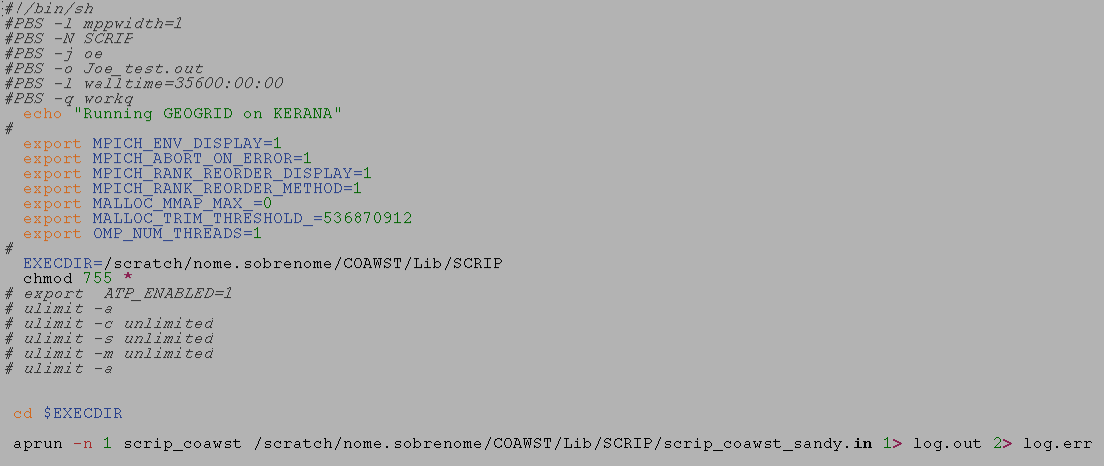
\includegraphics[width=0.65\textwidth]{scripqsub.png}
    \caption{\textit{qsub\_scrip.sh} file used to run SCRIP.}
    \label{qsubscripsh}
\end{figure}
\bigskip

 To start SCRIP, type:
\bigskip

\begin{bashcode}
qsub qsub_scrip.sh
\end{bashcode}
\bigskip

 At the end, the file \textit{scrip\_static.nc} will be created. Now put them in your project folder and you're done! COAWST is ready to run.
\bigskip

\section{Running your simulation}{{{{ }}}}
\bigskip

 Now, with everything ready, your project is ready to be started. Visit the section \textcolor{bleu_cite}{\ref{sandyexec}} to remember 
how to execute the project.